\section{SECCIÓN 2. GESTIÓN}
Esta sección describe cada elemento principal de la organización que influye en la calidad del software del proyecto Galería de Imágenes Segura con Detección de Esteganografía.

\subsection{2.1 ORGANIZACIÓN}
La buena práctica del software requiere un cierto grado de independencia para el grupo SQA. Esta independencia proporciona una fortaleza clave a SQA; es decir, SQA tiene la libertad, si la calidad del producto está en peligro, de informar esta posibilidad directamente por encima del nivel del proyecto.

La Figura 2-1 muestra la organización del proyecto en relación con las responsabilidades SQA.

\begin{figure}[H]
\centering
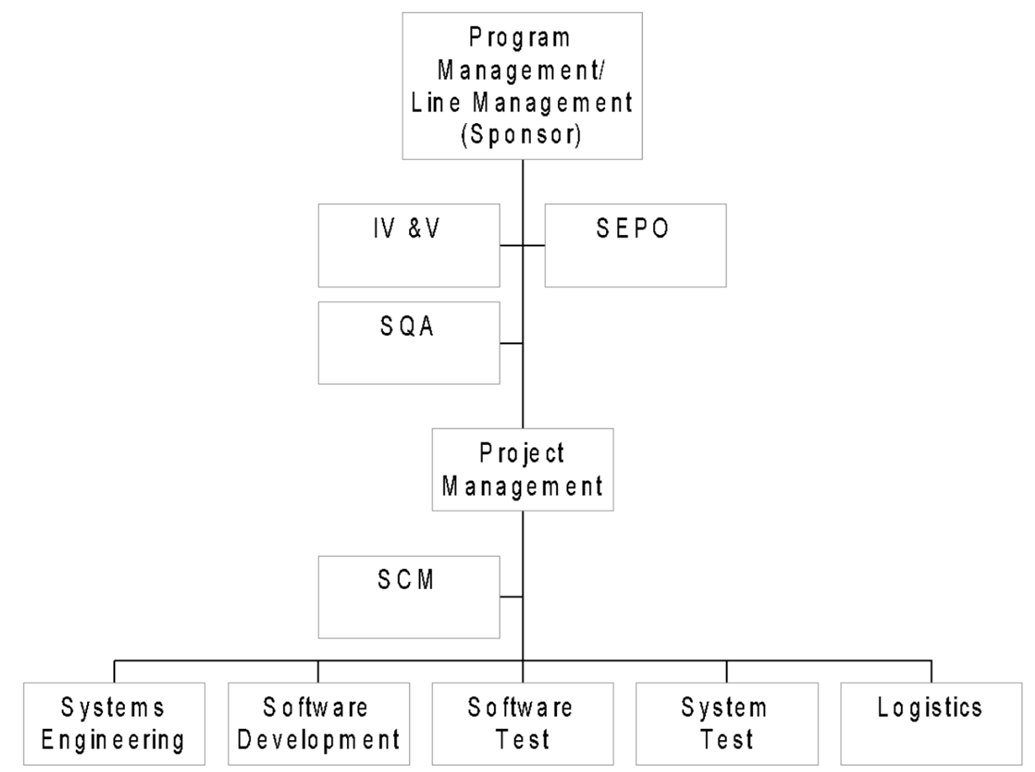
\includegraphics[width=0.9\textwidth]{images/imagen2.png}
\caption{Organización del Proyecto Galería de Imágenes Segura}
\label{fig:org}
\end{figure}

SQA es responsable de asegurar el cumplimiento de los requisitos de SQA delineados en este Plan SQA. La organización SQA asegura la calidad del software entregable y su documentación, el software no entregable, y los procesos de ingeniería utilizados para producir software.

A continuación se describen los grupos funcionales que influyen y controlan la calidad del software. La Tabla 3-2 del Proyecto define la matriz de responsabilidades asociada a estos grupos.

\begin{enumerate}
    \item \underline{Gerente SQA} --- es responsable de:
    \begin{enumerate}
        \item Implementar y mantener el Plan SQA del proyecto a lo largo de todo el ciclo de vida del desarrollo.
        \item Auditar los procesos de desarrollo de software para verificar el cumplimiento de los estándares, procedimientos y este Plan SQA.
        \item Revisar y evaluar los productos de software (entregables y no entregables) para asegurar la calidad.
        \item Registrar y reportar los resultados de las evaluaciones y auditorías de SQA a la Gestión del Proyecto.
        \item Coordinar las revisiones por pares de los productos de software según el Proceso de Revisión por Pares, referencia (n).
        \item Dar seguimiento a los hallazgos de calidad y verificar que las acciones correctivas se implementen y cierren.
        \item Revisar las mediciones de SQA (costo, cronograma, elementos de incumplimiento) y reportarlas mensualmente.
    \end{enumerate}


    \item \underline{Gerente de Proyecto} --- [Nombre] es responsable de:
    \begin{enumerate}
        \item Implementar el programa de calidad de acuerdo con los estándares del proyecto.
        \item Identificar las actividades SQA a ser realizadas por el Gerente SQA.
        \item Revisar y aprobar el Plan SQA del proyecto.
        \item Resolver y dar seguimiento a cualquier problema de calidad planteado por SQA.
        \item Identificar y asegurar los factores de calidad a implementar en el sistema y el software.
        \item Identificar, desarrollar y mantener documentos de planificación como el Plan de Desarrollo de Software, el Plan de Pruebas y este Plan SQA.
        \item Gestionar el cronograma, los recursos y la asignación de tareas del equipo.
    \end{enumerate}

    \item \underline{Ingeniería de Sistemas} --- es responsable de:
    \begin{enumerate}
        \item Revisar y comentar el Plan SQA del proyecto.
        \item Implementar el programa de calidad de acuerdo con este Plan SQA.
        \item Resolver y dar seguimiento a cualquier problema de calidad planteado por SQA relacionado con las actividades de ingeniería.
        \item Diseñar la arquitectura del sistema (backend Spring Boot, frontend React, persistencia PostgreSQL).
        \item Identificar e implementar los factores de calidad del sistema (seguridad, rendimiento, integridad).
        \item Definir las interfaces entre componentes y verificar su correcta integración.
    \end{enumerate}

    \item \underline{Diseño/Desarrollo de Software} -- es responsable de:
    \begin{enumerate}
        \item Revisar y comentar el Plan SQA del proyecto.
        \item Implementar el programa de calidad de acuerdo con este Plan SQA.
        \item Resolver y dar seguimiento a cualquier problema de calidad planteado por SQA relacionado con el diseño y desarrollo del software.
        \item Implementar las prácticas, procesos y procedimientos de codificación definidos en la Sección 5.
        \item Realizar pruebas unitarias del código implementado y registrar resultados.
        \item Participar en revisiones de código y corregir defectos identificados.
    \end{enumerate}

    \item \underline{Pruebas} --- es responsable de:
    \begin{enumerate}
        \item Revisar y comentar el Plan SQA del proyecto.
        \item Implementar el programa de calidad de acuerdo con este Plan SQA.
        \item Resolver y dar seguimiento a cualquier problema de calidad planteado por SQA relacionado con las pruebas.
        \item Ejecutar los casos de prueba definidos en el Plan de Pruebas (CP01--CP38) y registrar resultados.
        \item Verificar que los factores de calidad se implementen en el sistema, específicamente en el software.
        \item Generar informes de cobertura (JaCoCo), análisis estático (SonarQube, Qlty) y pruebas de seguridad (OWASP ZAP).
    \end{enumerate}
\end{enumerate}

\subsection{2.2 RECURSOS}

\subsubsection{ Instalaciones y Equipos}

\begin{table}[H]
\centering
\caption{Recursos del Proyecto}
\label{tab:resources}
\begin{tabular}{|p{4cm}|p{5cm}|p{5cm}|}
\hline
\textbf{RECURSO} & \textbf{DESCRIPCIÓN} & \textbf{USO} \\
\hline
GitHub & Repositorio remoto del proyecto & Control de versiones (SCM), gestión de issues, revisiones de código \\
\hline
Docker \& Docker Compose & Entorno de contenedores & SonarQube (análisis estático), ClamAV (escaneo de malware), despliegue del backend \\
\hline
Vercel & Plataforma de despliegue & Hospedaje del frontend React (producción) \\
\hline
Java 21 + Maven (mvnw) & Runtime y herramienta de compilación & Desarrollo y compilación del backend Spring Boot \\
\hline
Node.js 20+ \& npm & Runtime y gestor de paquetes & Desarrollo del frontend React, ejecución de pruebas Cypress \\
\hline
PostgreSQL 14+ & Sistema de gestión de bases de datos & Persistencia del sistema (producción) \\
\hline
H2 Database & Base de datos en memoria & Ejecución de pruebas unitarias e integración (perfil test) \\
\hline
Entorno de desarrollo local & IDE, editor de código & Codificación, depuración, revisiones por pares \\
\hline
\end{tabular}
\end{table}

\subsubsection{ Personal}

\begin{table}[H]
\centering
\caption{Estructura del Equipo del Proyecto}
\label{tab:team}
\begin{tabular}{|p{3.5cm}|p{4cm}|p{2cm}|p{3.5cm}|}
\hline
\textbf{ROL} & \textbf{NOMBRE} & \textbf{CÉDULA} & \textbf{PORCENTAJE DE ESFUERZO} \\
\hline
Gerente SQA & Gabriel López & [Cédula] & 100\% \\
\hline
Ingeniería de Sistemas & Mateo Llumigusín & [Cédula] & 100\% \\
\hline
Pruebas & Fernando Tipán & [Cédula] & 100\% \\
\hline
Pruebas & Kevin Asmal & [Cédula] & 100\% \\
\hline
Pruebas & Marcelo Pareja & [Cédula] & 100\% \\
\hline
\end{tabular}
\end{table}

\subsubsection{ Calificaciones del Personal}

El Gerente de SQA deberá estar familiarizado y poder aplicar los estándares y pautas enumerados en la Sección 1.6. Además, el Gerente de SQA deberá estar familiarizado con la calidad del software, las actividades relacionadas con el desarrollo de software y el análisis estructurado, diseño, codificación y pruebas.

El personal de Desarrollo de Software deberá tener experiencia en Java/Spring Boot (backend) y JavaScript/React (frontend), así como conocimiento de los estándares de codificación definidos en la Sección 5.

El personal de Pruebas deberá estar familiarizado con las herramientas de prueba definidas en la Sección 8 (JUnit, Cypress, JaCoCo, SonarQube, OWASP ZAP, JMeter, Lighthouse) y con la ejecución y documentación de casos de prueba.